% !TEX program = xelatex
\documentclass[oneside,master]{zjuthesis}
% 默认为单面模式,如需打印请把oneside换为twoside,博士请将master换为doctor
%==============================================================
%==============================================================

%自己需要增加什么 package 或修改什么设置的话,都放在这里吧。
\usepackage{enumerate}
\usepackage[perpage,symbol]{footmisc}
\setfnsymbol{wiley}
\usepackage{hypbmsec}
\usepackage{dsfont}
\usepackage{listings}
\usepackage{xcolor}

\newcommand{\tabincell}[2]{\begin{tabular}{@{}#1@{}}#2\end{tabular}}

%==============================================================
%==============================================================
\begin{document}

%==============================================================
%==============================================================
%这部分是论文封面、题名页需要的信息,请根据《研究生学位论文编写规则》自行修改

%论文分类号
  \renewcommand{\zjuclass}{TM888} 

%论文密级
  \renewcommand{\zjusecurity}{}
 
\renewcommand{\zjutitlec}{***********}%中文论文题目
\renewcommand{\zjutitlecb}{}%中文论文题目第二行,若无请留空
\renewcommand{\zjutitlecc}{}%中文论文题目第三行,若无请留空
\renewcommand{\zjutitlee}{Comparative Study on Primary School}%英文论文题目
\renewcommand{\zjutitleeb}{Mathematics Textbook Between}%英文论文题目第二行,若无请留空
\renewcommand{\zjutitleec}{Chinese and American}%英文论文题目第三行,若无请留空

%作者姓名
  \renewcommand{\zjuauthor}{袁淳} 

%作者学号
  \renewcommand{\zjuauthorid}{21935006}

%指导教师 
  \renewcommand{\zjumentor}{杨勋年}

%合作导师(如果有的话请取消注释)
  %\renewcommand{\zjumentorco}{}

%专业名称
  \renewcommand{\zjumajor}{应用数学}

%研究方向
  \renewcommand{\zjusubject}{数学课程}

%所在学院
  \renewcommand{\zjuschool}{数学科学学院}

%提交日期
  \renewcommand{\zjuapprovaldate}{二〇一九年四月}

%答辩日期
  \renewcommand{\zjudefencedatec}{二〇一九年六月}
  \renewcommand{\zjudefencedatee}{June 2019}

%论文评阅人(格式:姓名 ~ 职称 ~ 单位)
  \renewcommand{\zjurevieweronec}{陈某某 ~ 教授 ~ XX大学}
  \renewcommand{\zjurevieweronee}{Moumou Chen ~Prof. ~XX University}

  \renewcommand{\zjureviewertwoc}{张某某 ~ 教授 ~ XX大学}
  \renewcommand{\zjureviewertwoe}{Moumou Zhang ~Prof. ~XX University}

  \renewcommand{\zjureviewerthreec}{李某某 ~ 教授 ~ XX大学}
  \renewcommand{\zjureviewerthreee}{Moumou Li ~Prof. ~XX University }

  \renewcommand{\zjureviewerfourc}{吴某某 ~ 教授 ~ XX大学}
  \renewcommand{\zjureviewerfoure}{Moumou Wu ~Prof. ~XX University}

  \renewcommand{\zjureviewerfivec}{杨某某 ~ 教授 ~ XX大学}
  \renewcommand{\zjureviewerfivee}{Moumou Yang ~Prof. ~XX University}

%答辩委员会(姓名\职称\单位)
  \renewcommand{\zjucommitteemainc}{郑某某 ~ 教授 ~ 浙江大学}
  \renewcommand{\zjucommitteemaine}{Moumou Zheng~ Prof. ~Zhejiang University}

  \renewcommand{\zjucommitteeonec}{郑某某 ~ 教授 ~ 浙江大学}
  \renewcommand{\zjucommitteeonee}{Moumou Zheng ~Prof. ~Zhejiang University}

  \renewcommand{\zjucommitteetwoc}{刘某某 ~ 教授 ~ 浙江大学}
  \renewcommand{\zjucommitteetwoe}{Moumou Liu ~Prof. ~Zhejiang University}

  \renewcommand{\zjucommitteethreec}{程某某 ~ 教授 ~ 浙江大学}
  \renewcommand{\zjucommitteethreee}{Moumou Chen ~Prof. ~Zhejiang University}

  \renewcommand{\zjucommitteefourc}{杨某某 ~ 教授 ~ 浙江大学}
  \renewcommand{\zjucommitteefoure}{Moumou Yang ~Prof. ~Zhejiang University}

  \renewcommand{\zjucommitteefivec}{吴某某 ~ 教授 ~ 浙江大学}
  \renewcommand{\zjucommitteefivee}{Moumou Wu ~Prof. ~Zhejiang University}


%==============================================================
% 这部分除了“取舍”外,不需要自己修改,必要信息都已在上面设置。
\xiaosi
  %封面
  %%% 封面

\thispagestyle{empty}

\begin{tabbing}
\Songti\xiaosi 分类号: \= \underline{\makebox[4cm]{\xiaosi\zjuclass}} \= \hspace{4cm} \= \Songti\xiaosi 单位代码:\underline{\makebox[3cm]{10335}} \\
\Songti\xiaosi 密 \quad 级: \> \underline{\makebox[4cm]{\zjusecurity}} \> \> \Songti\xiaosi 学 \quad\quad 号:\underline{\makebox[3cm]{\zjuauthorid}}
\end{tabbing}

\vspace{5mm}

\begin{center}
   
\includegraphics[width=52mm]{images/zjdx}%浙江大学
\end{center}

\ifthenelse{\equal{\zjudegree}{D}}{\centerline{\Songti\xiaoyi 博士学位论文}}{}
\ifthenelse{\equal{\zjudegree}{M}}{\centerline{\Songti\xiaoyi 硕士学位论文}}{}

\vspace{4mm}

\begin{center}
  
\includegraphics[width=21mm]{images/standxb.png}%校徽
\end{center}

\vspace{8mm}

\begin{tabbing}
\Songti\sanhao\bfseries 中文论文题目:\=\hspace{-4mm}\xunderline[112mm]{\linespread{1.1}\bfseries\Fangsong\xiaoer\centerline\zjutitlec}
\ifthenelse{\equal\zjutitlecb{}}{}{\\[2mm]\>\hspace{-4mm}\xunderline[112mm]{\linespread{1.1}\bfseries\Fangsong\xiaoer\centerline\zjutitlecb}}
\ifthenelse{\equal\zjutitlecc{}}{}{\\[2mm]\>\hspace{-4mm}\xunderline[112mm]{\linespread{1.1}\bfseries\Fangsong\xiaoer\centerline\zjutitlecc}}
\\[2mm]\Songti\sanhao\bfseries 英文论文题目:\>\hspace{-4mm}\xunderline[112mm]{\linespread{1.1}\bfseries\sanhao\TNR\centerline\zjutitlee}
\ifthenelse{\equal\zjutitleeb{}}{}{\\[2mm]\>\hspace{-4mm}\xunderline[112mm]{\linespread{1.1}\bfseries\sanhao\TNR\centerline\zjutitleeb}}
\ifthenelse{\equal\zjutitleec{}}{}{\\[2mm]\>\hspace{-4mm}\xunderline[112mm]{\linespread{1.1}\bfseries\sanhao\TNR\centerline\zjutitleec}}
\end{tabbing}

\vspace{15mm}

\begin{tabbing}
\hspace{25mm} \Songti\sihao 申 \hspace{-2mm} \= \Songti\sihao 请人姓名: \= \underline{\makebox[7cm]{\sihao\zjuauthor}} \\[2mm]
              \> \Songti\sihao 指导教师: \> \underline{\makebox[7cm]{\sihao\zjumentor}} \\[2mm]
              %\> \Songti\sihao合作导师: \> \underline{\makebox[6cm]{\sihao\zjumentorco}} \\[2mm]
              \> \Songti\sihao 专业名称: \> \underline{\makebox[7cm]{\sihao\zjumajor}} \\[2mm]
              \> \Songti\sihao 研究方向: \> \underline{\makebox[7cm]{\sihao\zjusubject}} \\[2mm]
              \> \Songti\sihao 所在学院: \> \underline{\makebox[7cm]{\sihao\zjuschool}}
\end{tabbing}

\vspace{10mm}

\begin{tabbing}
\hspace{30mm} \= \Songti\xiaosan\bfseries 论文提交日期: \= \underline{\makebox[49mm]{\Songti\xiaosan\bfseries\zjuapprovaldate}}
\end{tabbing}

\ifthenelse{\equal{\zjuside}{T}}{%
  %\newpage\mbox{}%
  \thispagestyle{empty}}{}

  %中文题名页
  %%% 中文提名页

\newpage
\thispagestyle{empty}

\vspace{5mm}

\begin{center}
\xunderline[115mm]{\linespread{1.1}\xiaoer\Fangsong\bfseries\centerline\zjutitlec}
\ifthenelse{\equal\zjutitlecb{}}{}{\\[2mm]\xunderline[115mm]{\linespread{1.1}\xiaoer\Fangsong\bfseries\centerline\zjutitlecb}}
\ifthenelse{\equal\zjutitlecc{}}{}{\\[2mm]\xunderline[115mm]{\linespread{1.1}\xiaoer\Fangsong\bfseries\centerline\zjutitlecc}}
\end{center}

\vspace{5mm}

\begin{center}
  
\includegraphics[width=21mm]{images/standxb.png}
\end{center}

\vspace{3mm}

\begin{tabbing}
\hspace{30mm} \= \Songti\xiaosan\bfseries 论文作者签名: \= \underline{\makebox[5cm]{}} \\[8mm]
              \> \Songti\xiaosan\bfseries 指导教师签名: \> \underline{\makebox[5cm]{}}
\end{tabbing}

\vspace{8mm}

\begin{tabbing}
\hspace{10mm} \Songti\sihao 论文 \hspace{-2.6mm} \= \Songti\sihao 评阅人~1: \= \underline{\makebox[9cm]{\sihao\zjurevieweronec}} \\
              \> \Songti\sihao 评阅人~2: \> \underline{\makebox[9cm]{\sihao\zjureviewertwoc}} \\
              \> \Songti\sihao 评阅人~3: \> \underline{\makebox[9cm]{\sihao\zjureviewerthreec}} \\
              \> \Songti\sihao 评阅人~4: \> \underline{\makebox[9cm]{\sihao\zjureviewerfourc}} \\
              \> \Songti\sihao 评阅人~5: \> \underline{\makebox[9cm]{\sihao\zjureviewerfivec}}
\end{tabbing}

\vspace{8mm}

\begin{tabbing}
\hspace{5mm}\Songti\sihao 答辩委员 \hspace{-2.6mm} \= \Songti\sihao 会主席: \= \underline{\makebox[9cm]{\sihao\zjucommitteemainc}} \\
          \>    \Songti\sihao~委员~1: \> \underline{\makebox[9cm]{\sihao\zjucommitteeonec}} \\
          \>    \Songti\sihao~委员~2: \> \underline{\makebox[9cm]{\sihao\zjucommitteetwoc}} \\
          \>    \Songti\sihao~委员~3: \> \underline{\makebox[9cm]{\sihao\zjucommitteethreec}} \\
          \>    \Songti\sihao~委员~4: \> \underline{\makebox[9cm]{\sihao\zjucommitteefourc}} \\
          \>    \Songti\sihao~委员~5: \> \underline{\makebox[9cm]{\sihao\zjucommitteefivec}}
\end{tabbing}

\vspace{8mm}

\begin{tabbing}
\hspace{34mm} \= \Songti\sihao 答辩日期: \= \underline{\makebox[5cm]{\Songti\sihao\zjudefencedatec}} \\
\end{tabbing}

\ifthenelse{\equal{\zjuside}{T}}{%
  %\newpage\mbox{}%
  \thispagestyle{empty}}{}

  %英文题名页
  %%% 英文标题页

\newpage
\thispagestyle{empty}

\vspace{5mm}

\begin{center}
\xunderline[115mm]{\linespread{1.1}\xiaoer\TNR\bfseries\centerline\zjutitlee}
\ifthenelse{\equal\zjutitleeb{}}{}{\\[2mm]\xunderline[115mm]{\linespread{1.1}\xiaoer\Fangsong\bfseries\centerline\zjutitleeb}}
\ifthenelse{\equal\zjutitleec{}}{}{\\[2mm]\xunderline[115mm]{\linespread{1.1}\xiaoer\Fangsong\bfseries\centerline\zjutitleec}}
\end{center}

\vspace{5mm}

\begin{center}
  
\includegraphics[width=21mm]{images/standxb.png}
\end{center}

\vspace{-6mm}

\begin{tabbing}
\hspace{20mm} \= \sanhao\bfseries Supervisor's signature: \= \underline{\makebox[5cm]{}}\kill \\
              \> \hspace{7mm} \sanhao\bfseries Author's signature: \> \underline{\makebox[5cm]{}} \\[5mm]
              \> \sanhao\bfseries Supervisor's signature: \> \underline{\makebox[5cm]{}}
\end{tabbing}

\vspace{8mm}

\begin{tabbing}
\sihao External Reviewers: \= \underline{\makebox[10.8cm]{\sihao\zjurevieweronee}} \\
                    \> \underline{\makebox[10.8cm]{\sihao\zjureviewertwoe}} \\
                    \> \underline{\makebox[10.8cm]{\sihao\zjureviewerthreee}} \\
                    \> \underline{\makebox[10.8cm]{\sihao\zjureviewerfoure}} \\
                    \> \underline{\makebox[10.8cm]{\sihao\zjureviewerfivee}} \\[8mm]
\sihao Examining Committe Chairperson: \= \\
\hspace{41mm} \= \underline{\makebox[10.8cm]{\sihao\zjucommitteemaine}} \\
\sihao Examining Committe Members: \= \\
\hspace{41mm} \= \underline{\makebox[10.8cm]{\sihao\zjucommitteeonee}} \\
             \> \underline{\makebox[10.8cm]{\sihao\zjucommitteetwoe}} \\
             \> \underline{\makebox[10.8cm]{\sihao\zjucommitteethreee}} \\
             \> \underline{\makebox[10.8cm]{\sihao\zjucommitteefoure}} \\
             \> \underline{\makebox[10.8cm]{\sihao\zjucommitteefivee}}
\end{tabbing}

\vspace{6mm}

\begin{tabbing}
\hspace{28mm} \= \sihao Date of oral defence: \underline{\makebox[5cm]{\sihao\zjudefencedatee}}
\end{tabbing}

\ifthenelse{\equal{\zjuside}{T}}{%
  %\newpage\mbox{}%
  \thispagestyle{empty}}{}
 % 硕士论文请根据需要取舍。
  %独创性声明
  %% 独创性声明

\newpage
\thispagestyle{empty}

{\songti\xiaosi

\begin{center}
\xiaoer 浙江大学研究生学位论文独创性声明
\end{center}

\vspace{2mm}

本人声明所呈交的学位论文是本人在导师指导下进行的研究工作及取得的研究成果。除了文中特别加以标注和致谢的地方外,论文中不包含其他人已经发表或撰写过的研究成果,也不包含为获得\underline{\Kaiti\bfseries\sihao ~浙江大学~}或其他教育机构的学位或证书而使用过的材料。与我一同工作的同志对本研究所做的任何贡献均已在论文中作了明确的说明并表示谢意。

\begin{tabbing}
\hspace{0.5\linewidth} \= \hspace{0.5\linewidth} \kill \\
学位论文作者签名: \> 签字日期: \quad\quad\quad 年 \quad\quad 月 \quad\quad 日
\end{tabbing}

\vspace{10mm}

\begin{center}
\xiaoer 学位论文版权使用授权书
\end{center}

\vspace{2mm}

本学位论文作者完全了解\underline{\Kaiti\bfseries\sihao ~浙江大学~}有关保留、使用学位论文的规定,有权保留并向国家有关部门或机构送交本论文的复印件和磁盘,允许论文被查阅和借阅。本人授权\underline{\Kaiti\bfseries\sihao ~浙江大学~}可以将学位论文的全部或部分内容编入有关数据库进行检索和传播,可以采用影印、缩印或扫描等复制手段保存、汇编学位论文。

(保密的学位论文在解密后适用本授权书)

\begin{tabbing}
\hspace{0.5\linewidth} \= \hspace{0.5\linewidth} \kill \\
学位论文作者签名: \> 导师签名: \\[5mm]
签字日期: \quad\quad\quad 年 \quad\quad 月 \quad\quad 日 \> 签字日期: \quad\quad\quad 年 \quad\quad 月 \quad\quad 日
\end{tabbing}

}

\ifthenelse{\equal{\zjuside}{T}}{%
  %\newpage\mbox{}%
  \thispagestyle{empty}}{}


  \frontmatter
  \pagenumbering{Roman}

  %勘误页
  %\input{errata}  % 请根据需要取舍。
  %致谢
  %致谢
\chapter*{\centerline{致\quad 谢}}
\chaptermark{致谢}
\addcontentsline{toc}{chapter}{致谢}
\vspace{1cm}

% 感谢我的爹,感谢我的妈,感谢那个亲爱的他。
感谢杨勋年老师对我的信任,给足了我自由发展的空间,让我按着自己的兴趣前行。

感谢CAD实验室的冯旭东同学,让我克服了对无穷无尽的未知Bug,红色Error,黄色Warning的恐惧,
让我知道我只要磨下去,我是能够把代码跑起来的。

感谢我自己,在遇到困难的时候没有松口;在面对一大堆未知的知识时选择了挖下去;
在面对“赚不赚钱”的质疑时坚持了自己的兴趣。

感谢我的运气,我的努力还是让一些人看见,让我可以继续做我感兴趣的方向。
  \newpage
  %序言
  %\input{preface} % 请根据需要取舍。
  %中文摘要
  %% 中文摘要
\chapter*{\centerline{摘\quad 要}}
\chaptermark{摘要}
\addcontentsline{toc}{chapter}{摘要}

\vspace{1em}
物质点法是一种求解偏微分方程的数值计算方法。近年来,物质点法在物理仿真领域取得了巨大的进步,从电影行业,地球物理,到材料科学都带来了巨大的革新,展现出其强大的生命力。
得益于其算法框架的包容性,多种物理现象能够同时在一个系统里求解,带来一些过去从未成功模拟过的结果。然而,物质点法相较于其他
算法,在流体解算上面带来许多不真实的现象,尤其是在流体粘性和表面张力的部分。由于物质点法对于物质的表示形式是粒子,难以定义表面,这给表面张力
的模拟带来了巨大的困难,同时因为物质点法本身对时间步长要求严格,为了得到和表面张力耦合稳定的结果,经常在方程中加入阻尼项以及使用隐式格式,而这
更加剧了物质点法本身数值粘性,往往使最后的模拟结果不尽如人意。

本文研究了一种在物质点法框架下计算流体表面张力的方法,其主要思想是利用点云重构流体表面用于计算表面张力,
同时改进了表面粒子和内部粒子插值格式以及表面张力项的离散格式,提高了辛积分的稳定性,其相比于纯隐式格式降低了数值耗散,缓解了流体粘性问题。
本文的主要工作如下:

    (一)结合物质点法的计算流水线,提出了新的基于渐进迭代法的流体表面重构方法。
    利用物质点法本身的数据结构,在不增大内存负担的情况下,做到高速并行。同时给出相应的法向估计算法,相比于直接
    通过梯度或者网格估计法向,计算效率更高。    

    (二)基于工作(一)改进了表面张力数值计算格式。通过采样重建得到的表面网格,获取表面积分粒子用于计算表面张力,并通过新的数值离散方式,给出的表面张力项易于实现。同时给出
    嵌入内部粒子的方式,让表面张力能够更快地传导到内部粒子,提高了辛积分格式的稳定性。

\vspace{1em}

\noindent{\bfseries\Fangsong 关键词:}~~物质点法; 流体模拟; 表面张力; 隐式曲面重建 

  %英文摘要
  %% 英文摘要
\chapter*{\centerline{Abstract}}
\chaptermark{Abstract}
\addcontentsline{toc}{chapter}{Abstract}

\vspace{1em}
Since 2001,with the implementation of Basic Education Curriculum RefoHn,in our
reform process,the policy of”many editions under one stander”makes our country’S
math education a deep—going transformation.,SO study textbooks become focal point in
theory and practice math education.Internal research on American math education contains:
studying for standards,the actual class local studies,lack of total and complete analyzing
the American school math textbook.



\vspace{1em}

\textbf{Keywords:}~~Education; Chinese; American; Mathematics in Primary School; Textbook


%==============================================================
%这部分不需要自己修改。


  %插图和附表清单
  \listoffigures
  \chaptermark{图目录}
  \addcontentsline{toc}{chapter}{图目录}
  \listoftables
  \chaptermark{表目录}
  \addcontentsline{toc}{chapter}{表目录}
  %术语表
  % \printnomenclature
  % \chaptermark{术语表}
  %目次页
  \tableofcontents
  \addtocontents{toc}{\protect\chaptermark{目录}}
  \addtocontents{toc}{\protect\contentsline {chapter}{\protect\makebox[\linewidth]{目录\hfill}\vspace{-2em}}{}}
  \mainmatter

%==============================================================

  
\chapter{绪论}
\label{chap_int}
\section{问题背景}
计算机模拟几乎在所有的工程领域的一个重要工具,从土木工程、地球物工程、生物医学工程这些大型工程领域,到服装设计、家具设计这些生活周边,再到
游戏行业,电影特效这些文化领域处处都有计算机模拟的身影。计算机模拟不单单只是解决一些极其复杂难以实验,难以分析的问题,它也在替代一些昂贵耗时的物理实验,
给设计人员一些基础的直观信息。

目前主要的模拟方法以及一些商业化的工业模拟都是在有限元~\cite{1942Variational}的框架下实现的。尽管有限元方法已经理论成熟,并且早已经在学术界和工业界广泛的使用,
但是当用来求解一些大形变问题,拓扑变化问题时有限元便显得捉襟见肘,虽然这些问题可以使用重新网格化或者自适应网格来解决,但是网格处理本身就是一个复杂的问题,最后由此带来的便是
算法的鲁棒性问题,以及算法的性能也会大打折扣。

在电影特效行业以及游戏行业,经常遇到的问题便是大形变以及多物理场耦合问题,这也导致传统的有限元方法难以应对。然而,电影特效与游戏行业本身对模拟精度的要求并不是那么高,对于这些
对精度没有太高要求的问题,人们转而不再单纯的使用网格来表示物体,更灵活的粒子表示方法进入了学者们的视野。近年来,在电影特效界,首当其冲粒子表示方法的便是物质点法,该方法很大程度
解决了有限元大形变以及拓扑变化难的缺点,同时由于其加入了空间背景网格参与求解,使其对物理场建模有着极大的灵活性,在应对复杂多样的物理现象时,常常可以使用物质点法作为切入点。但是,
在流体模拟中,物质点法相对于专门为流体计算设计的方法并不完善,效果也相差甚远,如流体粘性,表面张力等效应都没有得到很好的表现,而这也使得多物理场模拟在涉及流体的时候,往往并不能
很全面的表现出流体的特性,或给人以不真实感。
\section{相关工作}
\subsection{物质点法}
Walt Disney工作室在2013年成功对雪的模拟~\cite{stomakhin2013material}将物质点法带到了图形学领域,同时在《冰雪奇缘》这部电影中大放异彩。此时的物质点法在图形学领域还仅仅是用于
模拟沙泥这类粘状的物质,但是其方便多物理场耦合的特性已经吸引了众多学者的注意,从Ram模拟粘性的牙膏、海绵、泡沫~\cite{2015foams}这类符合物质点法特性的材料,到Chengfanfu等人提出了APIC,在物质点法中加入仿射项~\cite{jiang2015affine}改进物质点法,
使其能够模拟粘性较低的流体,再到Gergely等人改进塑性的屈服模型~\cite{klar2016drucker},沙粒模拟也加入到物质点法能够模拟的范畴。之后Wang将有限元与物质点法相结合,让弹性体~\cite{2019WangDuctile}能够方便的
实现破碎效果,同时改进物质点法本身的数值粘性带来的碰撞不真实感。在有了这么多的针对单种物质模拟的基础工作之后,人们开始着手于多物理场,如在2017年Tampubolu等人的~\cite{tampubolon2017multi}对水和沙子耦合的模拟,Chengfanfu等人对布料沙子以及头发
织物~\cite{jiang2017anisotropic}的模拟,这些复杂的场景带来了惊人的视觉效果。在2019年,物质点法开始向着“生活”迈进,Mengyuan等人~\cite{Ding2019}首先将热转换、弹塑性、气体压强、流体压强、流体蒸发这些现象耦合在一起,成功的在计算机中模拟了烤曲奇饼干、烤面包、夹心面包、
水果风干等效果,展现出物质点法框架巨大的包容性。除了发掘物质点法优势之外,也有学者在改进物质点法本身的劣势,比如物质点法模拟流体时,经常表现出数值粘性,给人一种胶水质感。ChuYuan等~\cite{fu2017polynomial}人针对流体所展现的粘性,继续改进物质点法的粒子网格对流过程,
通过APIC,使物质点法下的流体展现出更多细节,同时更好的保留速度信息,大大的降低了流体本身的粘性。Yu等人~\cite{fang2020iq}针对物质点法流体和固体耦合时,由固体表面计算时带来的数值粘性做出了改进,成功的解决了流体流过固体表面出现粘连的问题。

\subsection{流体表面张力模拟}
\subsection{表面重构}
\section{研究内容}

\section{本章小结}

%introduction
  \chapter{连续介质力学} \label{chap2}
\section{引言}
连续介质力学是本文构建控制方程的理论基础。
基于连续介质力学,我们刻画流体以及流体表面,并从两个
视角来描述物体运动,以此构建动力学方程。为了构建完整的控制方程,我们还需要给出本构模型,
即形变与应力的关系,这里我们给出对应的流体的弱可压缩模型以及表面张力模型。

\section{欧拉视角下的动力学}
欧拉视角,即物理量的定义域为$\mathbb{R}^3$,对物体的刻画由空间中的密度场给出。与拉格朗日视角的区别我们将在2.3小节中给出。

\subsection{欧拉视角下的质量守恒定律}
记$\rho : \mathbb{R}^3 \times \mathbb{R} \rightarrow \mathbb{R}$ 为空间中随时间变化的密度场,
$v : \mathbb{R}^3 \times \mathbb{R} \rightarrow \mathbb{R}^3$ 为空间中随时间变化的速度场,此处默认向量为列向量。
\begin{figure}[htbp]
    \centering
    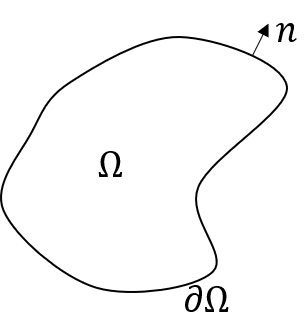
\includegraphics[scale=0.5]{./images/image1.png}
    \caption[区域符号示例]{区域符号示例}
    \label{fig:domain}
\end{figure}

现在考虑一个闭区域$\Omega$,$\Omega$的边界记为$\partial \Omega$,边界上的外法向记为
$n$,同时假定$\rho$ 和 $v$在 $\Omega$的一个开邻域内足够光滑。根据质量守恒,容易得到$\Omega$上质量的
变化率为$\partial \Omega$上质量的流出率和流入率之和。即
\begin{equation}
    \begin{split}
        \frac{d}{dt}\int_{\Omega} \rho(x,t)dx &= -\int_{\partial \Omega} \rho v \cdot n ds \\
        \int_{\Omega} \frac{\partial}{\partial t} \rho (x,t)dx &= -\int_{\Omega} div(\rho v)dx\nonumber\\
    \end{split}
\end{equation}
如果$\rho$在$\mathbb{R}^3$上都能达到足够光滑,那么由$\Omega$的任意性,可知
\begin{equation}
    \frac{\partial}{\partial t}\rho (x,t) + div(\rho v) = 0
\end{equation}

\subsection{欧拉视角下的动量守恒定律}
现在考虑闭区域$\Omega$上的动量变化。根据连续介质力学中的牛顿运动定律~\cite{gonzalez2008first},闭区域$\Omega$上的动量变化可以分为三部分,
第一部分为物质流入流出$\Omega$导致的动量变化,第二部分为作用在$\Omega$边界上的力导致的动量变化,第三部分为作用在$\Omega$内部物质上的力(一般为重力)产生的作用变化。
即
\begin{equation}
    \frac{d}{dt} \Big |_{t = t_0} \int_{\Omega} \rho v dx = -\int_{\partial \Omega} \rho v (v\cdot n) ds + \int_{\partial \Omega} \sigma \cdot n ds + \int_{\Omega} \rho g dx
\end{equation}
在(2.2)式中,$g$为重力加速度,$\sigma$为Cauthy应力~\cite{gonzalez2008first}。特别地,$\sigma$是一个三阶对称矩阵,其对称性来源于角动量守恒~\cite{marsden1994mathematical},我们将在2.4节中从另一个角度说明其对称性。

由于(2.2)式中$\Omega$选择的任意性,我们有
\begin{equation}
    \frac{\partial}{\partial t} \Big |_{t = t_0}(\rho v) = -div(\rho v^{T}v) + div(\sigma) + \rho g
\end{equation}

矩阵函数散度$div$定义如下:
\begin{equation}
    \begin{split}
        div &: C^1(\mathbb{R}^3;\mathbb{R}^{3\times 3}) \rightarrow C^1(\mathbb{R}^3;\mathbb{R}^3)\\
        &div(A)_i := \sum_j \partial_j A_{ij}\nonumber\\
    \end{split}
\end{equation}

(2.2)式变形为
\begin{equation}
    \frac{\partial}{\partial t} \Big |_{t = t_0}(\rho v) + div(\rho v^{T}v) = div(\sigma) + \rho g
\end{equation}


\section{拉格朗日视角下的动力学}
在上一节中,本文根据质量守恒和动量守恒得到了两个方程(方程(2.1)与方程(2.4)),非常重要的一点是,上述方程并没有使用任何
有关自然状态--材料在不施加外力的静止状态--的信息。在之后的章节中,我们将假定,$t=0$是处于自然状态,并且只考虑$t \ge 0$ 的情况。

假定在自然状态下($t = 0$),材料占据的空间为$\Omega_0 \subset \mathbb{R}^3$,此时也称$\Omega_0$为参考构型。对于任意给定的$t\in (0,+\infty)$,
此时材料占据的空间为$\Omega_t \subset \mathbb{R}^3$,相对于参考构型$\Omega_0$,称$\Omega_t$为当前构型。

拉格朗日视角和欧拉视角的区别主要是函数的定义域。在上一节中,我们所有函数的定义域都在$\mathbb{R}^3$上,而本节我们将把视角限制在材料上,例如对于任意时刻$t$,
有$\Omega_t$上的实值函数,$f(\cdot,t) :\Omega_t \rightarrow \mathbb{R} $。

\subsection{形变映射,形变梯度,速度}
为了描述材料相对于参考构型发生的形变,我们引入形变映射 $$\phi:\Omega_0 \times [0,+\infty) \rightarrow \mathbb{R}^3$$
形变映射同时也给出了物体的运动轨迹。
为了方便,我们记$\phi_t (x) = \phi(x,t)$,实际上我们还假定$\{ \phi_t(x): t\in \mathbb{R}\}$构成了一个单参数变换群,并且关于$t$至少二阶光滑,关于$X$至少有连续的一阶导数。

有了形变映射,我们可以引入对局部形变的刻画,即形变梯度$F(X,t):=\frac{\partial \phi_t(X)}{\partial X}$。实际上,形变梯度$F(X,t)$还可以视为$X$处切空间的映射,即
$$F(X,t):T_X \Omega_0 \rightarrow T_x \Omega_t$$
对于任意的$\partial_X \in T_X \Omega_0$, $\partial_x = F(X,t)[\partial_X] \in \Omega_t$,
即形变梯度将$X$点的切向量$\partial_X$经过平移起始点,旋转方向,拉伸长度后得到$x$点的切向量$\partial_x$,如图2.2所示。
\begin{figure}[htbp]
    \centering
    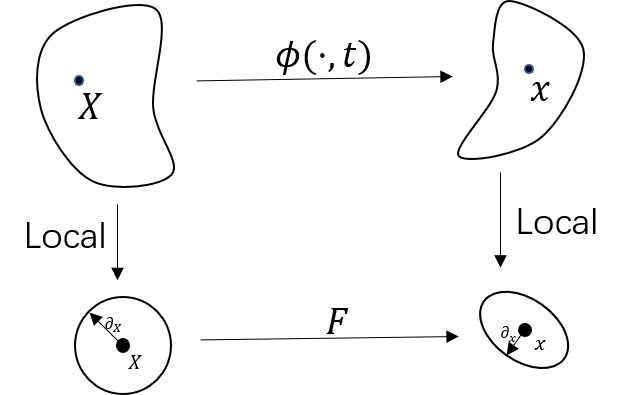
\includegraphics[scale=1.0]{./images/image2.png}
    \caption[形变与形变梯度]{形变与形变梯度}
    \label{fig:deformation gradient}
\end{figure}

同样的,形变映射作为单参数变换群,自然的导出速度的定义$V(X,t):= \frac{\partial \phi_t(X)}{\partial t}$。 值得注意的是,$V(X,t)$的定义域是在$\Omega_0$上,其值域
是一个起始点在$\Omega_t$上的一个三维列向量,其与欧拉视角下定义的速度关系为$V(X,t) = v(\phi_t(X),t)$,如果记$x = \phi_t(X)$,则$V(X,t) = v(x,t)$。

考察$F$关于时间的一阶导
\begin{equation}
    \begin{split}
        \frac{d}{dt}F(X,t) &= \frac{d}{dt}\frac{\partial}{\partial X}\phi_t\\
        &= \frac{\partial}{\partial X} \frac{d}{dt} \phi_t\\
        &= \frac{\partial}{\partial X} V(X,t)\\
        &= \frac{\partial v(\phi_t(X),t)}{\partial x}\frac{\partial \phi_t}{\partial X}\\
        &= \frac{\partial v(x,t)}{\partial x}\frac{\partial \phi_t}{\partial X}\\
        &= \nabla v \cdot F\nonumber
    \end{split}
\end{equation}
整理后我们得到$F$和$v$的关系
\begin{equation}
    \dot{F} = \nabla v \cdot F
\end{equation}


\subsection{拉格朗日视角下的质量守恒}
在引入了形变$\phi_t$之后,很自然的有$\hat{\Omega}_t = \{\phi_t(X):X\in \hat{\Omega}_0 \subset \Omega_0 \}$(简记为$\phi_t(\hat{\Omega}_0)$),且$\hat{\Omega}_t \subset \Omega_t$,
根据质量守恒,形变不会影响质量,即
$$\int_{\hat{\Omega}_0} \rho(x,0)dx = \int_{\hat{\Omega}_t} \rho(x,t)dx = \int_{\phi_t(\hat{\Omega}_0)} \rho(x,t)dx$$
如果我们将$\hat{\Omega}_t$的质量记为$M[\hat{\Omega}_t]$,则有$\frac{d}{dt}M[\hat{\Omega}_t] = 0$。而
\begin{equation}
    \begin{split}
        \frac{d}{dt} \int_{\phi_t(\hat{\Omega}_0)} \rho(x,t)dx &= \frac{d}{dt} \int_{\hat{\Omega}_0} \rho(\phi_t(X),t) det(F(X,t))dX\\
        &= \int_{\hat{\Omega}_0} \frac{d}{dt} [\rho(\phi_t(X),t) det(F(X,t))] dX \\
        &= 0\nonumber
    \end{split}
\end{equation}

记 $R(X,t):=\rho(\phi_t(X),t)$,$J(X,t):=det(F(X,t))$, 则根据$\hat{\Omega}_0$的任意性,有$\frac{d}{dt}[R(X,t)J(X,t)] = 0$,即
\begin{equation}
    R(X,t)J(X,t) = R(X,0)
\end{equation}
(2.6)式即为拉格朗日视角下的质量守恒方程。
\subsection{拉格朗日视角下的动量守恒}
在拉格朗日视角下,$\hat{\Omega}_{0}$的动量变化可以表示为作用在$\hat{\Omega}_{0}$边界上的力以及作用在$\hat{\Omega}_{0}$
内部的力之和。即
\begin{equation}
    \begin{split}
        \frac{d}{dt}\Big |_{t = t_0}\int_{\hat{\Omega}_0}R(X,0)V(x,t)dX = \int_{\partial \hat{\Omega}_{0}} P \cdot N dS + \int_{\hat{\Omega}_{0}} R(X,0) g dX
    \end{split}
\end{equation}
上式实际上对于任意的$\hat{\Omega}_0$成立,因此有以下
\begin{equation}
    R(X,0)\frac{\partial}{\partial t} V(X,t) = DIV(P) + Rg
\end{equation}
此处$DIV$是$\Omega_0$上的散度算子,为了与$\Omega_t$上进行区分记为大写。其中$P$是应力的另一种表述形式,称为First Piola–Kirchhoff应力~\cite{gonzalez2008first},其满足$\int_{\partial \hat{\Omega}_{0}} P \cdot N dS = \int_{\partial \hat{\Omega}_{t}} \sigma \cdot n ds$
我们将在下一节本构关系中更详细的给出$P$的计算方式以及与$\sigma$的关系。 

当然拉格朗日视角与欧拉视角下的动量守恒实际是等价的,我们接下来根据~\cite{gonzalez2008first}来说明其等价性,并且整理出一个更简洁的表达形式。
\begin{equation}
    \begin{split}
        \frac{d}{dt}\Big |_{t = t_0}\int_{\hat{\Omega}_0}R(X,0)V(x,t)dX &= \frac{d}{dt}\Big |_{t = t_0} \int_{\hat{\Omega}_0}R(X,t)v(\phi_t(X),t)J(X,t)dX\\
        &=\int_{\hat{\Omega}_0} \frac{d}{dt}\Big |_{t = t_0} [\rho(\phi_t(X),t)v(\phi_t(X),t)J(X,t)]dX\\
        &=\int_{\hat{\Omega}_0} \frac{d}{dt}\Big |_{t = t_0} [\rho(\phi_t(X),t)v(\phi_t(X),t)J(X,t)]dX\\
        &=\int_{\hat{\Omega}_0} v(\phi_{t_0}(X),t_0)\frac{d}{dt}\Big |_{t = t_0}[\rho(\phi_t(X),t) J(X,t)] \\
        &+ \rho(\phi_{t_0}(X),{t_0})J(X,t_0)\frac{d}{dt}\Big |_{t = t_0} v(\phi_{t_0}(X),t_0) dX\nonumber\\
        &=\int_{\hat{\Omega}_0}v(\phi_{t_0}(X),t_0)\frac{d}{dt}\Big |_{t = t_0}R(X,0) \\
        &+ \rho(\phi_{t_0}(X),{t_0})J(X,t_0)\frac{d}{dt}\Big |_{t = t_0} v(\phi_{t}(X),t)dX\\
        &=\int_{\hat{\Omega}_0}\rho(\phi_{t_0}(X),{t_0})J(X,t_0)\frac{d}{dt}\Big |_{t = t_0} v(\phi_{t}(X),t)dX\\
        &=\int_{\hat{\Omega}_{t_0}}\rho(x,t_0)\frac{d}{dt}\Big |_{t = t_0} v(\phi_{t,t_0}(x),t)dx\nonumber
    \end{split}
\end{equation}
这里$\phi_{t,t_0} = \phi_t \cdot \phi_{t_0}^{-1}$,带入(2.7)中就有
\begin{equation}
    \begin{split}
        \int_{\hat{\Omega}_{t_0}}\rho(x,t_0)\frac{d}{dt}\Big |_{t = t_0} v(\phi_{t,t_0}(x),t)dx = \int_{\hat{\Omega}_{t_0}} div(\sigma) dx + \int_{\hat{\Omega}_{t_0}} \rho g dx\nonumber
    \end{split}
\end{equation}
这里由于$\hat{\Omega}_{t_0}$为$\Omega_t$内的任意闭区域,因此
$$\rho(x,t_0)\frac{d}{dt}\Big |_{t = t_0} v(\phi_{t,t_0}(x),t) = div(\sigma) + \rho g$$

其中$$\frac{d}{dt}\Big |_{t = t_0} v(\phi_{t,t_0}(x),t) = \frac{\partial}{\partial t}\Big |_{t = t_0}v(x,t) + \sum_i \frac{\partial \phi_{t,t_0}^i}{\partial t}  \cdot \frac{\partial}{\partial x_i}v(x,t_0) = \frac{\partial}{\partial t}\Big |_{t = t_0}v(x,t) + v^T\nabla v$$
这里$\phi_{t,t_0}^i$为$\phi_{t,t_0}$的第$i$个分量。
此处引入材料时间导数$\frac{D}{Dt}f := \frac{\partial}{\partial t} f + v\nabla f $,将其代入上式中整理得
\begin{equation}
    \begin{split}
        \rho \frac{Dv}{Dt} = div(\sigma) + \rho g
    \end{split}
\end{equation}
该方程实际与(2.4)式等价,由于其更简洁的表述形式,我们之后将称(2.9)式为欧拉视角下的动量守恒。
$$\frac{\partial}{\partial t}(\rho v) + div(\rho v^{T}v) = div(\sigma) + \rho g$$
可考察方程的左端项
\begin{align*}
    \frac{\partial}{\partial t}(\rho v) + div(\rho v^{T}v) & = \rho \frac{\partial}{\partial t} v + v \frac{\partial}{\partial t} \rho + \rho v^T\nabla v + v div(\rho v)                           \\
                                                           & = \rho (\frac{\partial}{\partial t} v + v^T\nabla v) + v(\frac{\partial}{\partial t} \rho + div(\rho v))     & \text{第二项为质量守恒} \\
                                                           & = \rho \frac{Dv}{Dt}
\end{align*}
带入即知,(2.4)式是(2.8)式的展开。

\section{本构关系}
在前两节中,我们在动量守恒方程中引入了应力项,其决定了速度如何随着时间变化。本节我们将通过形变来给出
应变张量,其中应变张量和形变的函数关系被称为本构关系。事实上,本构关系直接决定了我们模拟的物体会表现出何种特质。

流体被认为是一种不可压缩的物质,用数学的语言就是说其形变梯度$F$满足$det(F)\equiv 1$,然而在实践中,为了更好的配合物质点法的使用,
我们从要求$det(F)\equiv 1$转变为使用形变能量密度来惩罚形变对体积的影响,$W(F):= \frac{\lambda}{2} (det(F) - 1)^2$。可以发现,对任意的$F\in \mathbb{R}^{3\times 3}, U\in SO_3$,始终有$W(UF) = W(F)$,
该特性被称为旋转不变性,根据诺特定理~\cite{takhtadzhian2008quantum},如果能量密度是旋转不变的,那么所得到的系统是角动量守恒的。

在有了能量密度函数,我们推导能量密度变化量和形变梯度的变化量之间的关系
\begin{equation}
    \begin{split}
        \delta W(F)&= \frac{\lambda}{2}\delta (det(F) - 1)^2\\
        &= \lambda (det(F) - 1) \delta(det(F) - 1)\\
        &= \lambda (det(F) - 1) \delta(det(F)) \nonumber\\
    \end{split}
\end{equation}
为了计算$\delta det(F)$,首先考察$\frac{d}{dt}\Big |_{t = 0}det(F + tI)$,由矩阵的特征多项式得
$$det(F + \epsilon I) = \epsilon ^n + \epsilon ^{n-1}Tr(F) + ... + det(F)$$
则等式两边同时除$\epsilon^n$得
$$det(\frac{1}{\epsilon}F + I) = 1 + \frac{1}{\epsilon} * Tr(F) + ... + \frac{1}{\epsilon^n} det(F)$$
此时将$t\neq 0$代入有
$$det(tF + I) = 1 + t Tr(F) + ... + t^ndet(F)$$
同时验证$t=0$可知上式恒成立。
因此$\frac{d}{dt}\Big |_{t = 0}det(tF + I) = tr(F)$,
现在对于任意的$t_0$以及$\mathbb{R}^{3 \times 3}$中通过$A(t_0)$(假设$A(t_0)$可逆)的一条光滑路径$A(t)$,我们有对应的通过$I$的路径
$A(t_0)^{-1}A(t)$,其对应的切向量为$A(t_0)^{-1}\frac{d}{dt}\Big |_{t=t_0}A(t)$,则
\begin{equation}
    \begin{split}
        \frac{d}{dt}\Big |_{t = t_0} det(A(t)) &= \lim_{h \to 0} \frac{det(A(t_0 + h)) - det(A(t_0))}{h}\\
        &=det(A(t)) \lim_{h\to 0} \frac{det(A(t_0)^{-1}A(t_0 + h)) -1}{h}\\
        &= det(A(t))tr(A(t_0)^{-1}\frac{d}{dt}\Big |_{t=t_0}A(t))\\
        &= det(A(t))A(t_0)^{-T}:\frac{d}{dt}\Big |_{t=t_0}A(t)
    \end{split}
\end{equation}
这里$A:B:=\sum_{i,j}A_{ij}B_{ij}$。

故$\delta det(F) = det(F) F^{-T}:\delta F$,代入$\delta W(F)$之中即有$$\delta W(F) = \lambda (det(F) - 1)det(F) F^{-T}:\delta F$$
其中$P = \lambda (det(F) - 1)det(F)F^{-T}$被称为First Piola–Kirchhoff应力,其与Cauthy应力$\sigma$的关系~\cite{marsden1994mathematical}为
$$J\sigma = PF^{T}$$
我们将在本小节最后给出该关系式的证明,代入可知柯西应力$\sigma = \lambda (det(F) - 1)I$。

这里的$W(F)$实际上只给出了物体的抗压缩性的性质,我们还需要给出表面张力的能量密度函数。根据~\cite{popinet2018numerical},表面能实际和物体表面积成正比,表面张力为表面能的梯度。那么我们首先可以得出
形变和表面能量的关系
\begin{equation}
    S(\phi_t) = k\int_{\phi_t (\partial \Omega_0)} ds
\end{equation}
为了更好的计算其梯度,我们对(2.11)式做一些处理。此处引入一些微分流形的记号~\cite{lee2013smooth},记$f^*$为$f$导出的拉回映射,$f_*$为推前映射,$ds,d\tilde{s}$分别为曲面$\partial \Omega_{t_0}, \partial \Omega_{t}$上的面积二形式,其为空间体积形式$dv$内乘法向的结果,
即$ds(X,Y) = dv(n,X,Y)$,我们记$ds = dv\odot n$,$ \tilde{p} = \phi_{t_0,t}(p)$,则对任意的$t \in[0, t_0),\tilde{X},\tilde{Y}\in T_{\tilde{p}}\Omega_t$有如下
\begin{equation}
    \begin{split}
        (\phi_{t_0,t}^*ds) (\tilde{X},\tilde{Y})& = (\phi_{t_0,t}^* (dv \odot n))(\tilde{X},\tilde{Y})\\
        &= ((\phi_{t_0,t}^* dv)\odot(\phi_{t_0,t}^* n))(\tilde{X},\tilde{Y})\\
        &= det(F(x;t_0,t))dv (<F^{-1}(x;t_0,t)n,\tilde{n}>\tilde{n} ,\tilde{X},\tilde{Y})\\
        &= det(F(x;t_0,t))<F^{-1}(x;t_0,t)n,\tilde{n}> dv(\tilde{n} ,\tilde{X},\tilde{Y})\\
        &= det(F(x;t_0,t))<n,F^{-T}(x;t_0,t)\tilde{n}>dv(\tilde{n} ,\tilde{X},\tilde{Y})
    \end{split}
\end{equation}
上式中$F(x;t_0,t) = \frac{\partial \phi_{t_0,t}(x)}{\partial x}$,$\tilde{n}$为$T_{\tilde{p}}\Omega_t$单位法向,$<\cdot,\cdot>$为空间内积,容易验证$F^{-T}(x;t_0,t)\tilde{n}$与$T_p\Omega_0$垂直,
故$<n,F^{-T}(x;t_0,t)\tilde{n}> = \Vert F^{-T}(x;t_0,t)\tilde{n}\Vert$, 即$\Vert F^{-T}(x;t_0,t)\tilde{n}\Vert n = F^{-T}(x;t_0,t)\tilde{n}$,那么有
$$(\phi_{t_0,t}^*ds) = det(F(x;t_0,t)) \Vert F^{-T}(x;t_0,t)\tilde{n}\Vert d\tilde{s}$$
则代入表面能表达式有
\begin{equation}
    \begin{split}
        S(\phi_{t_0}) &= k  \int_{\partial\Omega_{t_0}}ds\\
        &= k \int_{\phi_{t_0,t}(\partial\Omega_{t})} ds\\
        &= k \int_{\partial \Omega_t}  \phi_{t_0,t}^* ds\\
        &= k \int_{\partial \Omega_t} det(F(x;t_0,t)) \Vert F^{-T}(x;t_0,t)\tilde{n}\Vert d\tilde{s}\nonumber\\
    \end{split}
\end{equation}

至此,我们得到表面能的另一个表达形式
\begin{equation}
    \begin{split}
        S(\phi_{t_0}) = k \int_{\partial \Omega_t} det(F(x;t_0,t)) \Vert F^{-T}(x;t_0,t)\tilde{n}\Vert d\tilde{s}
    \end{split}
\end{equation}
(2.13)式将是表面张力离散化的基础。

最后,我们给出$J\sigma = PF^{T}$的证明,
\begin{align*}
    \int_{\partial \hat{\Omega}_{t}} \sigma \cdot n ds &= \int_{\phi_t (\partial \hat{\Omega}_{0})} \sigma\cdot n ds\\
    &= \int_{\partial \hat{\Omega}_0} \phi_t^*(\sigma\cdot n) (\phi_t^* ds)\\
    &= \int_{\partial \hat{\Omega}_0} \sigma\cdot n J \Vert F^{-T} N\Vert dS\\
    &= \int_{\partial \hat{\Omega}_0} \sigma F^{-T} \cdot F^{T}n J \Vert F^{-T} N\Vert dS\\
    &= \int_{\partial \hat{\Omega}_0} J\Vert F^{-T} N\Vert\sigma F^{-T} \cdot \frac{1}{\Vert F^{-T}N \Vert} N dS\\
    &= \int_{\partial \hat{\Omega}_0} J\sigma F^{-T} \cdot N dS\\
\end{align*}
而$\int_{\partial \hat{\Omega}_{0}} P \cdot N dS = \int_{\partial \hat{\Omega}_{t}} \sigma \cdot n ds$,因此$\int_{\partial \hat{\Omega}_0} J\sigma F^{-T} \cdot N dS = \int_{\partial \hat{\Omega}_0} P \cdot N dS$,
由于上式对任意$\partial \hat{\Omega}_0$成立,则$J\sigma F^{-T}= P$得$J\sigma = PF^{T}$。


\section{本章小结}
本章基于连续介质力学得到了一系列的控制方程
\begin{align*}
    &\frac{\partial}{\partial t}\rho (x,t) + div(\rho v) = 0 & \text{欧拉视角下的质量守恒方程} \\
    &R(X,t)J(X,t) = R(X,0) & \text{拉格朗日视角下的质量守恒方程} \\
    &\rho \frac{Dv}{Dt} = div(\sigma) + \rho g & \text{欧拉视角下的动量守恒方程}\\
    &R(X,0)\frac{\partial}{\partial t} V(X,t) = DIV(P) + Rg &\text{拉格朗日视角下的质量守恒方程}
\end{align*}

以上四个方程分别从两种视角分别等价的刻画了质量守恒和动量守恒,这两种视角也会在物质点法离散化的过程中体现出来。其次,通过整理得到
形变梯度更新方程~\cite{jiang2016material}
\begin{align*}
    \dot{F} = \nabla v \cdot F
\end{align*}
该方程将会在物质点法如何获得下一时刻的形变梯度中起到关键作用。最后,
我们给出了弱可压缩能量$W(F)=\lambda (J-1)^2$来刻画流体的特性,该能量也给出了First Piola–Kirchhoff应力和Cauthy应力的计算方式。
其次根据~\cite{popinet2018numerical}\cite{hyde2020implicit}得到表面能的另一个等价表达形式
$$S(\phi_{t_0}) = k \int_{\partial \Omega_{t_1}} det(F(x;t_0,t_1)) \Vert F^{-T}(x;t_0,t_1)\tilde{n}\Vert d\tilde{s}$$
该计算形式下,积分域不随着$\phi_{t_0}$变化而变化,为我们离散计算以及变分都带来了便利,而表面张力将由表面能变分获得,这一步我们将在离散化的过程(章节\ref{chap4})中来计算。







%literature
%==============================================================
%这也是个不需要自己修改的部分。

  \backmatter %结束章节自动编号

%参考文献(习惯使用bibtex的可以修改)
  \addcontentsline{toc}{chapter}{参考文献} % 解决目录中没有相应的参考文献的条目问题
  \chaptermark{参考文献}
  
\begin{thebibliography}{200}
    \bibitem{article1} Ernest P . The philosophy of mathematics education by Paul Ernest[J]. Social Epistemology.

    \bibitem{article2} Bishop A J. Mathematical enculturation: a cultural perspective on mathematics education[J]. Journal for Research in Mathematics Education, 1988, 20(4):195.


\end{thebibliography}


%附录
  %  \include{chapters/appe}

% 出版物
  % \input{chapters/publication}

% 作者简历
  \chapter*{\centerline{作者简历}}
\chaptermark{作者简历}
\addcontentsline{toc}{chapter}{作者简历}


袁淳,男,1996年,汉族,江西龙南人。2015年考入上海金融学院(金融数学专业),2019年本科毕业,获得经济学学士学位。2019年进入浙江大学数学科学学院应用数学专业研究生学习至今。

% \begin{enumerate}
%     \item 工作经历
%     \begin{itemize}
%         \item 20XX-20XX年,在XX公司XX部门XX岗位
%         \item 20XX-20XX年,在XX公司XX部门XX岗位
%     \end{itemize}

%     \item 参与的项目
%     \begin{itemize}
%         \item 20XX-20XX年,参与XXXX项目
%         \item 20XX-20XX年,负责XXXX项目
%     \end{itemize}

%     \item 攻读学位期间发表的论文
%     \begin{itemize}
%         \item 猪八戒, 猪悟能, 天蓬元帅, 等. 论流体食物的持久保存[D]. 硕士学位论文. 北京: 广寒宫大学, 2005
%     \end{itemize}

% \end{enumerate}

%==============================================================
%==============================================================
\end{document}
